\section{Supervisors}
 \frame{\sectionpage}


\begin{frame}{Supervisors}
1st supervisor:\newline
dr. Wieb Bosma\newline
Computer Algebra\newline
Faculty of Science - Radboud University Nijmegen\newline\newline
2nd supervisor and foreign component:\newline
dr. Marco Bonatto\newline
Quandle Theory\newline
Department of Mathematics and Computer Science - University of Ferrara
\end{frame}   


\section{Idea}
 \frame{\sectionpage}


\begin{frame}{Idea}

The idea is to develop a computer algebra module(of a computer algebra system) that can deal with quandles(and related algebraic structures).\newline \newline
The software tries to be a tool that ``standardises" computational research in a field where the creation of ad-hoc programs is still all too common while providing a tool that is useful to researchers. 
\end{frame}   




\section{Quandles}
 \frame{\sectionpage}


\begin{frame}{Quandles and other structures}

\begin{itemize}
    \item \textcolor{blue2}{A set: $\{\smiley, \frownie, \neutranie \}$, $\{1,2,3,4,5,6,7\}$, \dots}
    \item \textcolor{blue2}{An operation: $+$}
    \item \textcolor{blue2}{A few rules: \begin{itemize}
        \item[1] \textcolor{blue2}{$\smiley + \smiley = \smiley$}
        \item[2] \textcolor{blue2}{$\smiley = $} \textcolor{red2}{$\neutraniered$}  \textcolor{blue2}{$+ \frownie$}
        \item[3] \textcolor{blue2}{$(\smiley + \frownie) + \neutranie = (\smiley + \neutranie) + (\frownie + \neutranie)$ }
    \end{itemize}}
    
\end{itemize}

Other structures: \begin{itemize}
        \item \textcolor{violet2}{Rack}: it satisfies only rule 2 and rule 3.
        \item \textcolor{orange2}{Crossed set}, \textcolor{green2}{Prack}, \dots
    \end{itemize}
A Quandle can also be constructed from a \emph{mathematical} group(another algebraic structure).
\end{frame}   
 
 
 
 
 
 
 
 
\section{Origins and applications}
 \frame{\sectionpage}


\begin{frame}{Knots,  \dots}
\textcolor{violet2}{\emph{Q(trefoil) $= (a, b, c: a+b=c, b+c=a, c+a=b)$}}
\begin{figure}%
    \centering
    \subfloat[\centering fancy knot]{{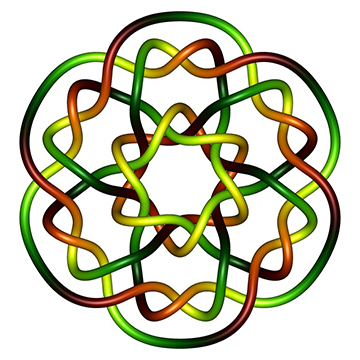
\includegraphics[scale=0.2]{Slides-March 8th/images/Fancy20Knot-small.jpg}}}
    \qquad
    \subfloat[\centering trefoil]{{
\includegraphics[scale=0.2]{Slides-March 8th/images/trefoil.png} }}%
    \qquad
    \subfloat[\centering knotted doughnut]{{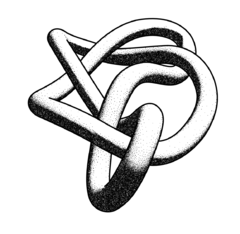
\includegraphics[scale=0.2]{Slides-March 8th/images/Knotted_torus2C_6_2.png}}}%
    
    
    \label{fig:example}%
\end{figure}
\begin{minipage}{1\textwidth}
    Knot theory has been used to study proteins and nucleic acids.\newline
    Distinguish knots. \newline
    Adapted to distinguish different topological types of proteins $\to$ Bondles.\newline
     Describe the relationship between a Lie group and its associated Lie algebra. \newline
    Set-theoretical solutions to the quantum Yang-Baxter equation in statistical mechanics.
     
\end{minipage}

\end{frame}   

\section{Computations and progress}
\frame{\sectionpage}
\begin{frame}{Representation}
\[M_Q = \begin{bmatrix}
\smiley & \neutranieblack & \frownie \\
\neutranieblack & \frownie & \smiley \\
\frownie & \smiley & \neutranieblack
\end{bmatrix}\]

\begin{itemize}
    \item[1] Each element of the set appears in the diagonal exactly once. 
    \item[2] Each column does not show a result more than once.
    \item[3] $M_Q[M_Q[\smiley,\frownie], \neutranieblack] = M_Q[M_Q[\smiley, \neutranieblack], M_Q[\frownie, \neutranieblack]]$
\end{itemize}

\end{frame}

\begin{frame}{Progress}

I am working with \textsc{Magma}\footnote{Wieb Bosma, John Cannon, and Catherine Playoust.  The Magma Algebra System I: The User Language. \textit{Journal of Symbolic Computation}, 24(3):235–265, 1997}.
\begin{itemize}
    \item I made a database of quandles \emph{potentially} available to a wider audience. 
    \item I implemented classes to work with some of the most popular families of quandles
    \item I implemented matrix-based algorithms to compute some basic results and obtained results compatible with those in the literature.
\end{itemize}

\end{frame}

\begin{frame}{Plans for the future}


\begin{itemize}
    \item Start diverging from Rig\footnote{L. Vendramin. Rig, a GAP package for racks, quandles and Nichols algebras.} by implementing more algorithms. 
    \item Explore the connection between group theory and quandle theory and implement algorithms that exploit this connection. 
    \item It would be nice to:
    \begin{itemize}
        \item Explore how the Library for Automated Deduction Research(see Prover9, an automated theorem prover, and Mace4, a model finder which can be used to find counterexamples to disprove a claim) could be integrated in my tool. 
        \item Explore alternative representations of knots, maybe based on graphs.
        \item Compute the fundamental quandle of (at least some) knots, using the representation mentioned above.
        
    \end{itemize}
    
\end{itemize}

\end{frame}